\documentclass[10pt,oneside]{article}
\usepackage[T1]{fontenc}
\usepackage[utf8]{inputenc}
% \usepackage{lmodern}
%\usepackage[adobe-utopia,uppercase=upright,greeklowercase=upright]{mathdesign}
\usepackage[adobe-utopia]{mathdesign}
%\usepackage{minionpro}
% \usepackage{pifont}
% \usepackage{amssymb}
\usepackage{amsmath}
\usepackage[francais]{babel}
% \usepackage[francais]{varioref}
\usepackage[dvips]{graphicx}

\usepackage{framed}
\usepackage[normalem]{ulem}
\usepackage{fancyhdr}
\usepackage{titlesec}
\usepackage{vmargin}
\usepackage{longtable}

\usepackage{ifthen}


%\usepackage{epsfig}
\usepackage{subfig}

\usepackage{multirow}
\usepackage{multicol} % Portions de texte en colonnes
\usepackage{flafter}%floatants après la référence



\usepackage{color}
\usepackage{colortbl}


\definecolor{gris25}{gray}{0.75}
\definecolor{bleu}{RGB}{18,33,98}
\definecolor{bleuf}{RGB}{42,94,171}
\definecolor{bleuc}{RGB}{231,239,247}
\definecolor{rougef}{RGB}{185,18,27}
\definecolor{rougec}{RGB}{255,230,231}
\definecolor{vertf}{RGB}{103,126,82}
\definecolor{vertc}{RGB}{220,255,191}

\newenvironment{rem}[1][\hsize]%
{%
    \def\FrameCommand
    {%
\rotatebox{90}{\textit{\textsf{Remarque}}} 
        {\color{bleuf}\vrule width 3pt}%
        \hspace{0pt}%must no space.
        \fboxsep=\FrameSep\colorbox{bleuc}%
    }%
    \MakeFramed{\hsize#1\advance\hsize-\width\FrameRestore}%
}%
{\endMakeFramed}%


\newenvironment{savoir}[1][\hsize]%
{%
    \def\FrameCommand
    {%
\rotatebox{90}{\textit{\textsf{Savoir}}} 
        {\color{bleuf}\vrule width 3pt}%
        \hspace{0pt}%must no space.
        \fboxsep=\FrameSep\colorbox{bleuc}%
    }%
    \MakeFramed{\hsize#1\advance\hsize-\width\FrameRestore}%
}%
{\endMakeFramed}%

\newenvironment{prob}[1][\hsize]%
{%
    \def\FrameCommand%
    {%
\rotatebox{90}{\textit{\textsf{ Problématique}}} 
        {\color{rougef}\vrule width 3pt}%
        \hspace{0pt}%must no space.
        \fboxsep=\FrameSep\colorbox{rougec}%
    }%
    \MakeFramed{\hsize#1\advance\hsize-\width\FrameRestore}%
}%
{\endMakeFramed}%

\newenvironment{obj}[1][\hsize]%
{%
    \def\FrameCommand%
    {%
\rotatebox{90}{\textit{\textsf{ $\;$}}} 
        {\color{rougef}\vrule width 3pt}%
        \hspace{0pt}%must no space.
        \fboxsep=\FrameSep\colorbox{rougec}%
    }%
    \MakeFramed{\hsize#1\advance\hsize-\width\FrameRestore}%
}%
{\endMakeFramed}%

\newenvironment{defi}[1][\hsize]%
{%
    \def\FrameCommand%
    {%
\rotatebox{90}{\textit{\textsf{Définition\\}}} 
        {\color{bleuf}\vrule width 3pt}%
        \hspace{0pt}%must no space.
        \fboxsep=\FrameSep\colorbox{bleuc}%
    }%
    \MakeFramed{\hsize#1\advance\hsize-\width\FrameRestore}%
}%
{\endMakeFramed}%


\newenvironment{hypo}[1][\hsize]%
{%
    \def\FrameCommand%
    {%
\rotatebox{90}{\textit{\textsf{Hypothèse\\}}} 
        {\color{bleuf}\vrule width 3pt}%
        \hspace{0pt}%must no space.
        \fboxsep=\FrameSep\colorbox{bleuc}%
    }%
    \MakeFramed{\hsize#1\advance\hsize-\width\FrameRestore}%
}%
{\endMakeFramed}%


\newenvironment{prop}[1][\hsize]%
{%
    \def\FrameCommand%
    {%
\rotatebox{90}{\textit{\textsf{Propriété\\}}} 
        {\color{bleuf}\vrule width 3pt}%
        \hspace{0pt}%must no space.
        \fboxsep=\FrameSep\colorbox{bleuc}%
    }%
    \MakeFramed{\hsize#1\advance\hsize-\width\FrameRestore}%
}%
{\endMakeFramed}%

\newenvironment{props}[1][\hsize]%
{%
    \def\FrameCommand%
    {%
\rotatebox{90}{\textit{\textsf{Propriétés\\}}} 
        {\color{bleuf}\vrule width 3pt}%
        \hspace{0pt}%must no space.
        \fboxsep=\FrameSep\colorbox{bleuc}%
    }%
    \MakeFramed{\hsize#1\advance\hsize-\width\FrameRestore}%
}%
{\endMakeFramed}%

\newenvironment{exemple}[1][\hsize]%
{%
    \def\FrameCommand%
    {%
\rotatebox{90}{\textit{\textsf{Exemple\\}}} 
        {\color{vertf}\vrule width 3pt}%
        \hspace{0pt}%must no space.
        \fboxsep=\FrameSep\colorbox{vertc}%
    }%
    \MakeFramed{\hsize#1\advance\hsize-\width\FrameRestore}%
}%
{\endMakeFramed}%

\newenvironment{resultat}[1][\hsize]%
{%
    \def\FrameCommand%
    {%
\rotatebox{90}{\textit{\textsf{Résultat\\}}} 
        {\color{rougef}\vrule width 3pt}%
        \hspace{0pt}%must no space.
        \fboxsep=\FrameSep\colorbox{rougec}%
    }%
    \MakeFramed{\hsize#1\advance\hsize-\width\FrameRestore}%
}%
{\endMakeFramed}%

\newenvironment{methode}[1][\hsize]%
{%
    \def\FrameCommand%
    {%
\rotatebox{90}{\textit{\textsf{Méthode\\}}} 
        {\color{rougef}\vrule width 3pt}%
        \hspace{0pt}%must no space.
        \fboxsep=\FrameSep\colorbox{rougec}%
    }%
    \MakeFramed{\hsize#1\advance\hsize-\width\FrameRestore}%
}%
{\endMakeFramed}%

\newenvironment{theo}[1][\hsize]%
{%
    \def\FrameCommand%
    {%
\rotatebox{90}{\textit{\textsf{Théorème\\}}} 
        {\color{rougef}\vrule width 3pt}%
        \hspace{0pt}%must no space.
        \fboxsep=\FrameSep\colorbox{rougec}%
    }%
    \MakeFramed{\hsize#1\advance\hsize-\width\FrameRestore}%
}%
{\endMakeFramed}%

\newenvironment{warn}[1][\hsize]%
{%
    \def\FrameCommand%
    {%
\rotatebox{90}{\textit{\textsf{Attention\\}}} 
        {\color{rougef}\vrule width 3pt}%
        \hspace{0pt}%must no space.
        \fboxsep=\FrameSep\colorbox{rougec}%
    }%
    \MakeFramed{\hsize#1\advance\hsize-\width\FrameRestore}%
}%
{\endMakeFramed}%

% \usepackage{pstricks}
%\usepackage{minitoc}
% \setcounter{minitocdepth}{4}

\setcounter{tocdepth}{2}

% \mtcselectlanguage{french} 

%\usepackage{draftcopy}% "Brouillon"
% \usepackage{floatflt}
\usepackage{psfrag}
%\usepackage{listings} % Permet d'insérer du code de programmation
\renewcommand{\baselinestretch}{1.2}

% Changer la numérotation des figures :
% ------------------------------------
% \makeatletter
% \renewcommand{\thefigure}{\ifnum \c@section>\z@ \thesection.\fi
%  \@arabic\c@figure}
% \@addtoreset{figure}{section}
% \makeatother
 


%%%%%%%%%%%%
% Définition des vecteurs %
%%%%%%%%%%%%
 \newcommand{\vect}[1]{\overrightarrow{#1}}

%%%%%%%%%%%%
% Définition des torseusr %
%%%%%%%%%%%%

 \newcommand{\torseur}[1]{%
\left\{{#1}\right\}
}

\newcommand{\torseurcin}[3]{%
\left\{\mathcal{#1} \left(#2/#3 \right) \right\}
}

\newcommand{\torseurstat}[3]{%
\left\{\mathcal{#1} \left(#2\rightarrow #3 \right) \right\}
}

 \newcommand{\torseurc}[8]{%
%\left\{#1 \right\}=
\left\{
{#1}
\right\}
 = 
\left\{%
\begin{array}{cc}%
{#2} & {#5}\\%
{#3} & {#6}\\%
{#4} & {#7}\\%
\end{array}%
\right\}_{#8}%
}

 \newcommand{\torseurcol}[7]{
\left\{%
\begin{array}{cc}%
{#1} & {#4}\\%
{#2} & {#5}\\%
{#3} & {#6}\\%
\end{array}%
\right\}_{#7}%
}

 \newcommand{\torseurl}[3]{%
%\left\{\mathcal{#1}\right\}_{#2}=%
\left\{%
\begin{array}{l}%
{#1} \\%
{#2} %
\end{array}%
\right\}_{#3}%
}

 \newcommand{\vectv}[3]{%
\vect{V\left( {#1} \in {#2}/{#3}\right)}
}


\newcommand{\vectf}[2]{%
\vect{R\left( {#1} \rightarrow {#2}\right)}
}

\newcommand{\vectm}[3]{%
\vect{\mathcal{M}\left( {#1}, {#2} \rightarrow {#3}\right)}
}


 \newcommand{\vectg}[3]{%
\vect{\Gamma \left( {#1} \in {#2}/{#3}\right)}
}

 \newcommand{\vecto}[2]{%
\vect{\Omega\left( {#1}/{#2}\right)}
}
% }$$\left\{\mathcal{#1} \right\}_{#2} =%
% \left\{%
% \begin{array}{c}%
%  #3 \\%
%  #4 %
% \end{array}%
% \right\}_{#5}}

%  ------------------------------------------
% | Modification du formatage des sections : | 
%  ------------------------------------------

% Grands titres :
% ---------------

\newcommand{\titre}[1]{%
\begin{center}
      \bigskip
      \rule{\textwidth}{1pt}
      \par\vspace{0.1cm}
      
      \textbf{\large #1}
      \par\rule{\textwidth}{1pt}
    \end{center}
    \bigskip
  }

% Supprime le numéro du chapitre dans la numérotation des sections:
% -----------------------------------------------------------------
\makeatletter
\renewcommand{\thesection}{\@arabic\c@section}
\makeatother


% \titleformat{\chapter}[display]
% {\normalfont\Large\filcenter}
% {}
% {1pc}
% {\titlerule[1pt]
%   \vspace{1pc}%
%   \Huge}[\vspace{1ex}%
% \titlerule]


%%%% Chapitres Comme PY Pechard %%%%%%%%%
% numéro du chapitre
\DeclareFixedFont{\chapnumfont}{OT1}{phv}{b}{n}{80pt}
% pour le mot « Chapitre »
\DeclareFixedFont{\chapchapfont}{OT1}{phv}{m}{it}{40pt}
% pour le titre
\DeclareFixedFont{\chaptitfont}{T1}{phv}{b}{n}{25pt}

\definecolor{gris}{gray}{0.75}
\titleformat{\chapter}[display]%
	{\sffamily}%
	{\filleft\chapchapfont\color{gris}\chaptertitlename\
	\\
	\vspace{12pt}
	\chapnumfont\thechapter}%
	{16pt}%
	{\filleft\chaptitfont}%
	[\vspace{6pt}\titlerule\titlerule\titlerule]

%%%%  Fin Chapitres Comme PY Pechard %%%%%%%%%


% Section, subsection, subsubsection sans serifs :
% % ----------------------------------------------

% \makeatletter
% \renewcommand{\section}{\@startsection{section}{0}{0mm}%
% {\baselineskip}{.3\baselineskip}%
% {\normalfont\sffamily\Large\textbf}}%
% \makeatother

\makeatletter
\renewcommand{\@seccntformat}[1]{{\textcolor{bleu}{\csname
the#1\endcsname}\hspace{0.5em}}}
\makeatother

\makeatletter
\renewcommand{\section}{\@startsection{section}{1}{\z@}%
                       {-4ex \@plus -1ex \@minus -.4ex}%
                       {1ex \@plus.2ex }%
                       {\normalfont\Large\sffamily\bfseries}}%
\makeatother
 
\makeatletter
\renewcommand{\subsection}{\@startsection {subsection}{2}{\z@}
                          {-3ex \@plus -0.1ex \@minus -.4ex}%
                          {0.5ex \@plus.2ex }%
                          {\normalfont\large\sffamily\bfseries}}
\makeatother
 
\makeatletter
\renewcommand{\subsubsection}{\@startsection {subsubsection}{3}{\z@}
                          {-2ex \@plus -0.1ex \@minus -.2ex}%
                          {0.2ex \@plus.2ex }%
                          {\normalfont\large\sffamily\bfseries}}
\makeatother
 
\makeatletter             
\renewcommand{\paragraph}{\@startsection{paragraph}{4}{\z@}%
                                    {-2ex \@plus-.2ex \@minus .2ex}%
                                    {0.1ex}%               
{\normalfont\sffamily\bfseries}}
\makeatother
 
\makeatletter
\renewcommand{\subparagraph}{\@startsection{subparagraph}{5}{\z@}%
                                       {-2ex \@plus-.1ex \@minus .2ex}%
                                       {0.1ex}%
				    {\normalfont\normalsize\sffamily\bfseries}}
\makeatletter
% \makeatletter
% \renewcommand{\subsection}{\@startsection{subsection}{1}{2mm}%
% {\baselineskip}{.3\baselineskip}%
% {\normalfont\sffamily\large\textbf}}%
% \makeatother
% 
% \makeatletter
% \renewcommand{\subsubsection}{\@startsection{subsubsection}{2}{4mm}%
% {\baselineskip}{.15\baselineskip}%
% {\normalfont\sffamily\large\textbf}}%
% \makeatother
% 
% \makeatletter
% \renewcommand{\paragraph}{\@startsection{paragraph}{3}{6mm}%
% {\baselineskip}{.15\baselineskip}%
% {\normalfont\sffamily\large\textbf}}%
% \makeatother
 
\setcounter{secnumdepth}{4}


%  --------
% | Marges |
%  --------


% \setmarginsrb{2.5cm}{1.5cm}{2.5cm}{2cm}{1cm}{1cm}{1cm}{1cm}
\setmarginsrb{1.5cm}{1cm}{1cm}{1.5cm}{1cm}{1cm}{1cm}{1cm}

% Changer les marges localement :
% -----------------------------
\newenvironment{changemargin}[2]{\begin{list}{}{%
\setlength{\topsep}{0pt}%
\setlength{\leftmargin}{0pt}%
\setlength{\rightmargin}{0pt}%
\setlength{\listparindent}{\parindent}%
\setlength{\itemindent}{\parindent}%
\setlength{\parsep}{0pt plus 1pt}%
\addtolength{\leftmargin}{#1}%
\addtolength{\rightmargin}{#2}%
}\item }{\end{list}}



\usepackage{pst-solides3d}
\usepackage{titletoc}
\titlecontents{chapter}[+3pc]
  {\addvspace{10pt}\sffamily\bfseries}
{\contentslabel[{\pscirclebox[fillstyle=solid,fillcolor=gray!25,
linecolor=gray!25,framesep=4pt]{\textcolor{white}{\thecontentslabel}}}]{2.5pc}}
  {}
  {\dotfill \normalfont\thecontentspage\ }

\titlecontents{section}[3pc]
  {\addvspace{2pt}\sffamily}
  {\contentslabel[\thecontentslabel]{1.8pc}}
  {}
  {\dotfill \normalfont\thecontentspage\ }

\titlecontents{subsection}[5pc]
  {\addvspace{2pt}\sffamily}
  {\contentslabel[\thecontentslabel]{1.8pc}}
  {}
  {\dotfill \normalfont\thecontentspage\ }

\titlecontents{subsubsection}[8pc]
  {\addvspace{2pt}\sffamily}
  {\contentslabel[\thecontentslabel]{3pc}}
  {}
  {\dotfill \normalfont\thecontentspage\ }
%{\;\titlerule\;\normalfont\thecontentspage\ }

\titlecontents{paragraph}[9pc]
  {\addvspace{2pt}\sffamily}
  {\contentslabel[\thecontentslabel]{3.5pc}}
  {}
  {\dotfill \normalfont\thecontentspage\ }





%Si le boolen xp est vrai : compilation pour xabi
%Sinon compilation Damien
\newboolean{xp}
\setboolean{xp}{true}

\newboolean{prof}
\setboolean{prof}{true}

\def\xxtitre{\ifthenelse{\boolean{xp}}{
CI 3 -- CIN : Étude du comportement cinématique des systèmes}{
}}

\def\xxsoustitre{\ifthenelse{\boolean{xp}}{
Chapitre 7 -- Le Torseur \\ Torseur cinématique -- Torseur des petits déplacements}{
}}


\def\xxauteur{\ifthenelse{\boolean{xp}}{
\noindent 2013 -- 2014 \\
Xavier \textsc{Pessoles}}{
}}


\def\xxpied{\ifthenelse{\boolean{xp}}{
CI 3 : CIN -- Cours \\
Ch 7 : Torseurs -- \ifthenelse{\boolean{prof}}{P}{E}%
}{
}}

\usepackage[%
    pdftitle={CIN : Cinématique du point},
    pdfauthor={Xavier Pessoles},
    colorlinks=true,
    linkcolor=blue,
    citecolor=magenta]{hyperref}


\usepackage{pifont}
\sloppy
\hyphenpenalty 10000


\begin{document}






% \makeatletter \let\ps@plain\ps@empty \makeatother
%% DEBUT DU DOCUMENT
%% =================




%------------- En tetes et Pieds de Pages ------------


\pagestyle{fancy}
\ifthenelse{\boolean{xp}}{%
\renewcommand{\headrulewidth}{0pt}}{%
\renewcommand{\headrulewidth}{0.2pt}} %pour mettre le trait en haut
%\renewcommand{\headrulewidth}{0.2pt}

\fancyhead{}
\fancyhead[L]{%
\ifthenelse{\boolean{xp}}{%
\noindent\begin{minipage}[c]{2.6cm}%

\includegraphics[width=2cm]{png/logo_ptsi.png}%
\end{minipage}%
}{%
\footnotesize{\textit{\textsf{Lycée François Premier}}}
}}

\ifthenelse{\boolean{xp}}{%
\fancyhead[C]{\rule{12cm}{.5pt}}}{
}


\fancyhead[R]{%
\noindent\begin{minipage}[c]{3cm}
\begin{flushright}
\footnotesize{\textit{\textsf{Sciences Industrielles \\ de l'ingénieur}}}%
\end{flushright}
\end{minipage}
}


\ifthenelse{\boolean{xp}}{%
\fancyhead[C]{\rule{12cm}{.5pt}}}{
}

\renewcommand{\footrulewidth}{0.2pt}

\fancyfoot[C]{\footnotesize{\bfseries \thepage}}
\fancyfoot[L]{%
\begin{minipage}[c]{.2\linewidth}
\noindent\footnotesize{{\xxauteur}}
\end{minipage}
\ifthenelse{\boolean{xp}}{}{%
\begin{minipage}[c]{.15\linewidth}

\includegraphics[width=2cm]{png/logoCC.png}
\end{minipage}}
}


\fancyfoot[R]{\footnotesize{\xxpied}}



\begin{center}
 \huge\textsc{\xxtitre}

\end{center}

\begin{center}
 \LARGE\textsc{\xxsoustitre}
\end{center}

\begin{savoir}
\textbf{Savoirs :}
\begin{itemize}
\item Mod-- C11.1 : déplacement des points d’un solide : repère lié à un solide, paramètres géométriques linéaires et angulaires définissant la position d'un solide par rapport à un autre, déplacements et petits déplacements d'un solide, torseur des petits déplacements;
\item Mod-- C11.3 : torseur cinématique caractérisant le mouvement d’un solide;
\item Mod--C11--S7 : écrire le torseur cinématique caractérisant le mouvement d’un solide.
\end{itemize}
\end{savoir}

%\begin{center}
%\begin{tabular}{ccc}
%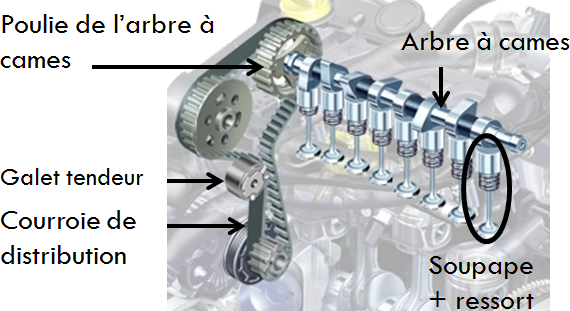
\includegraphics[height=3.5cm]{png/fig1} &
%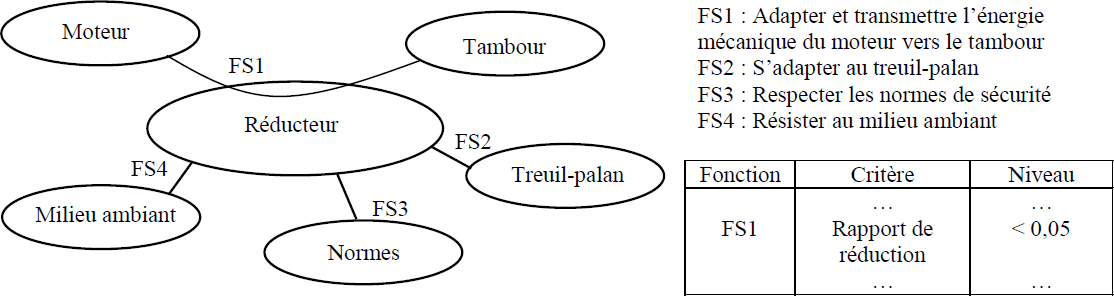
\includegraphics[height=3.5cm]{png/fig2}\\
%\textit{Modèle CAO d'un} & \textit{Modélisation par}\\
%\textit{arbre à came} & \textit{schéma cinématique}\\
%\end{tabular}
%\end{center}




\setlength{\parskip}{0ex plus 0.2ex minus 0ex}
 \renewcommand{\contentsname}{}
 \renewcommand{\baselinestretch}{1}

\tableofcontents

 \renewcommand{\baselinestretch}{1.2}
\setlength{\parskip}{2ex plus 0.5ex minus 0.2ex}

% \vspace{1cm}
\textit{Ce document est en évolution permanente. Merci de signaler toutes
erreurs ou coquilles.}


\section{Définitions}
\subsection{Torseurs}

\begin{defi}
Un torseur est constitué :
\begin{itemize}
\item d'un vecteur résultant $\vect{R}$;
\item d'un champ de vecteur $\mathcal{M}$ tel que pour tout couples de points $(A,B)$ on a : 
$$
\vect{\mathcal{M}_B} = \vect{\mathcal{M}_A} + \vect{BA} \wedge \vect{R}
$$
\end{itemize}
\end{defi}

Cette relation est appelée relation caractéristique des torseurs ou relation de Varignon.

Réciproquement, tout champ de vecteurs   qui vérifie la relation de Varignon pour tout couple de points $A$ et $B$, le vecteur $\vect{R}$ étant indépendant du bipoint $(A,B)$, est le champ de vecteurs d'un torseur.

\subsection{Expression en un point}
Si le champ de vecteurs est connu en un point, on peut le connaître en tout autre point en utilisant la relation de Varignon. Le torseur sera donc noté :
$$
\torseur{\mathcal{T}}=\torseurl{\vect{R}}{\vect{\mathcal{M}_A}}{}
\quad \text{au point }A, \quad 
\torseur{\mathcal{T}}=\torseurl{\vect{R}}{\vect{\mathcal{M}_B}}{}
\quad \text{au point }B \text{ avec } $$
$$
\vect{\mathcal{M}_B} = \vect{\mathcal{M}_A} + \vect{BA} \wedge \vect{R}
$$
On appelle :
\begin{itemize}
\item $\vect{R}$ la résultante du torseur;
\item $\vect{\mathcal{M}_A}$ le moment au point $A$ du torseur. Ce nom est donné par analogie avec la définition du moment en un point d'un pointeur;
\item $\vect{R}$ et $\vect{\mathcal{M}_A}$ sont les éléments de réduction du torseur. Ce sont deux vecteurs dont on peut faire une représentation graphique au point $A$ :
\end{itemize}

\begin{minipage}[c]{.47\linewidth}
\begin{center}
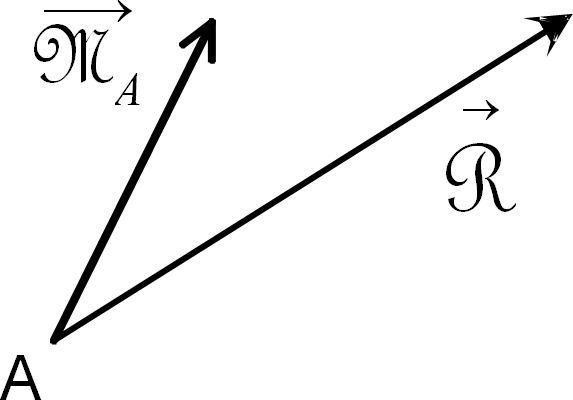
\includegraphics[width=.55\textwidth]{png/fig_1}
\end{center}
\end{minipage} \hfill
\begin{minipage}[c]{.47\linewidth}
\begin{center}
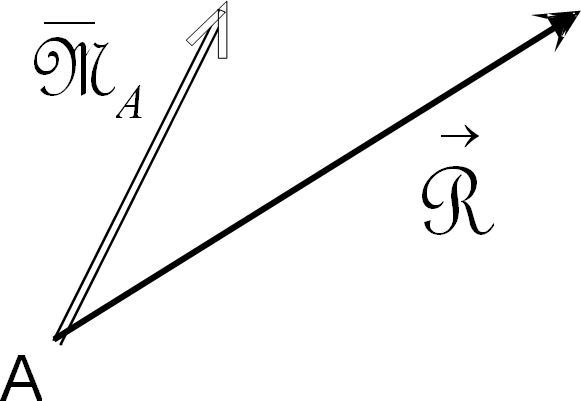
\includegraphics[width=.55\textwidth]{png/fig_02}
\end{center}
\end{minipage}

\subsection{Notation des torseurs}
Les torseurs sont utilisés en cinématique, statique, dynamique, métrologie, \textit{etc}. Le torseur est exprimé en général par une lettre majuscule significative de ce que l'on étudie. Cette lettre est encadrée d'accolades :
$$
\torseur{\mathcal{T}}, \torseur{\mathcal{V}(2/1)}, \torseur{\mathcal{F}(1\rightarrow 2)}, \torseur{\mathcal{U}(1/2)}, \torseur{\mathcal{C}(1/2)}, \torseur{\mathcal{D}(1/2)}
$$

\begin{itemize}
\item $\torseur{\mathcal{T}}$ : torseur général;
\item $\torseur{\mathcal{V}(2/1)}$ : torseur cinématique;
\item $\torseur{\mathcal{F}(1\rightarrow 2)}$ : torseur statique;
\item $\torseur{\mathcal{U}(1/2)}$ : torseur des petits déplacements;
\item $\torseur{\mathcal{C}(1/2)}$ : torseur cinétique;
\item $\torseur{\mathcal{D}(1/2)}$ : torseur dynamique.
\end{itemize}

Pour travailler sur ces torseurs, il est plus commode de le faire avec ses éléments de réduction. Le moment dépend du point d'expression. Il faut donc que la notation précise bien ce point :

$$
\torseur{\mathcal{T}} = \torseurl{\vect{R}}{\vect{\mathcal{M}_A}}
\quad \text{ou}\quad
\torseur{\mathcal{T}} =\torseur{\vect{R},\vect{\mathcal{M}_A}} 
$$

$$
\torseur{\mathcal{T}} = \torseurl{\vect{R}}{3\vect{x}+2\vect{y}}{A}
\quad \text{ou}\quad
\torseur{\mathcal{T}} =\torseur{\vect{R},3\vect{x}+2\vect{y}}_A
$$

Le point $A$ apparaît à l'intérieur ou à l'extérieur des accolades (par exemple, en indice à gauche ou à droite des accolades).

On peut aussi exprimer des éléments de réduction en projection sur une même base $\mathcal{B}$ et les écrire en colonne en précisant bien la base de projection :

$$
\torseur{\mathcal{T}}=\torseurcol{-6}{a}{1}{3}{2}{0}{A,\mathcal{B}}
$$

Les six composantes des éléments de réduction sont appelées les coordonnées pluckériennes du torseur.

\subsection{Invariants}
\begin{defi}
\textbf{Invariants}

On appelle invariants d'un torseur, des quantités qui restent constantes quel que soit le point de calcul.
\end{defi}

\begin{defi}
\textbf{Invariant vectoriel}

C'est la résultante du torseur.
\end{defi}

\begin{defi}
\textbf{Invariant scalaire}

$$
I = \vect{R} \cdot \vect{\mathcal{M}_A}
$$
\end{defi}

\begin{demo}
Exprimons $\vect{R}\cdot \vect{\mathcal{M}_B}$ , en utilisant le moment au point $A$ pour prouver que $I$ est bien invariant.

%\begin{eqnarray*}
$$
\vect{R}\cdot \vect{\mathcal{M}_B} %& 
=%& 
\vect{R}\cdot \left[\vect{\mathcal{M}_A}+\vect{BA}\wedge \vect{R}\right] = 
 \vect{R}\cdot \vect{\mathcal{M}_A}+ \underbrace{\vect{R}\cdot \left(\vect{BA}\wedge \vect{R}\right)}_{\vect{0}} %\\&
=%&
  \vect{R}\cdot \vect{\mathcal{M}_A} = I
$$%\end{eqnarray*}
\end{demo}

\subsection{Axe central}
\begin{defi}
Un point $K$ de l'espace est central pour le torseur $\torseur{T}$ si la résultante est colinéaire au moment en ce point :  
$$\vect{\mathcal{M}_K} =k \vect{R}$$
avec $k$ est appelé pas du torseur.

On démontre que l'ensemble des points centraux pour le torseur considéré est une droite appelée axe central. 

L'axe central est  parallèle à  $\vect{R}$.

\end{defi}

\subsection{Moment central}
\begin{defi}
Le moment central $\vect{\mathcal{M}_K}$ est la valeur du moment d'un torseur en un point central $K$.
\end{defi}
\begin{props}
%Soit $K'$ un autre point de l'axe central.
\begin{enumerate}
\item Le moment central est invariant pour deux points de l'axe central.
\item La norme du moment central est la norme minimale des moments. 
\end{enumerate}
\end{props}



\subsection{Représentation spatiale d'un torseur}

\begin{center}
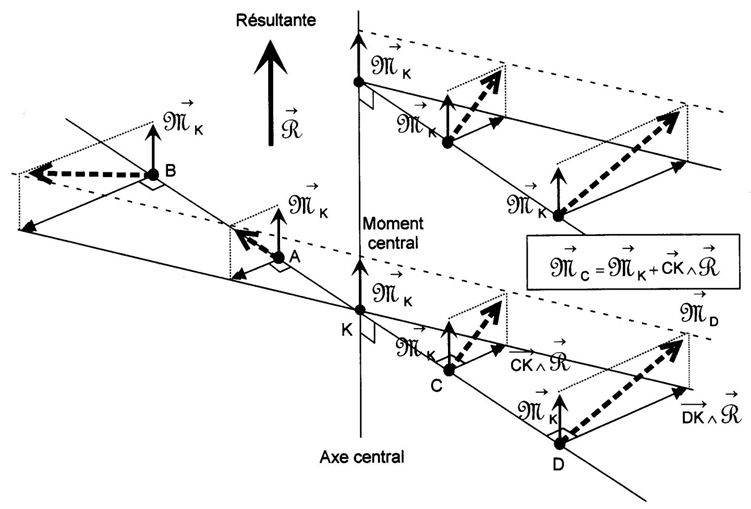
\includegraphics[width=.7\textwidth]{png/fig_03}
\end{center}


\subsection{\'Equiprojectivité du champ de vecteurs d'un torseur}
Pour un torseur on a $\vect{\mathcal{M}_B}=\vect{\mathcal{M}_A}+\vect{BA}\wedge\vect{R}$. Multiplions cette expression par le vecteur $\vect{AB}$.

\begin{eqnarray*}
\vect{\mathcal{M}_B} \cdot \vect{AB} & = &  \left(\vect{\mathcal{M}_A}+\vect{BA}\wedge\vect{R} \right)\cdot \vect{AB} =  
\vect{\mathcal{M}_A}\cdot \vect{AB} +  \underbrace{\left(\vect{BA}\wedge\vect{R} \right)\cdot \vect{AB}}_{\vect{0}}\\
&=& \vect{\mathcal{M}_A}\cdot \vect{AB}
\end{eqnarray*}
Ceci est la relation donnée lors du cours sur le calcul vectoriel pour un champ équiprojectif.

\section{Torseurs particuliers}
\subsection{Couple}
\begin{defi}
\textbf{Torseur couple}

Un torseur possédant une résultante nulle est appelé couple. 

$$
\torseur{\mathcal{T}} = \torseurl{\vect{0}}{\vect{\mathcal{M}_A}}{A}
$$
\end{defi}

\begin{prop}
Le moment d'un torseur couple est inchangé lorsqu'on l'exprime en un autre point.  On peut donc le noter plus simplement :
$
\torseur{\mathcal{T}} = \torseurl{\vect{0}}{\vect{\mathcal{M}}}{} 
$. (Dans ce cas, la notation du point n'est pas indispensable.)
\end{prop}

\begin{demo}
En appliquant la relation caractéristique des torseurs on trouve : 
$$
\vect{\mathcal{M}_B}=\vect{\mathcal{M}_A}+\vect{BA}\wedge\vect{R} =\vect{\mathcal{M}_A} + \vect{0}=\vect{\mathcal{M}_A}
$$

\end{demo}

\subsection{Glisseur}

\begin{defi}
\textbf{Glisseur}

Un glisseur est un torseur qui a sa résultante non nulle et son invariant scalaire nul.
\end{defi}

\begin{prop}
L'invariant scalaire nul entraîne : $I =\vect{\mathcal{M}_K}\cdot \vect{R} = 0$.   
\end{prop}

\begin{demo}
 Montrons que le moment central est nul :

Si $K$ est un point central $\vect{\mathcal{M}_K} = k \vect{R}$.
 En conséquence, $I=k\vect{R}\cdot\vect{R}= 0$ et donc $k=0$. $\vect{\mathcal{M}_K}$ est donc égal au vecteur nul.


\end{demo}
En un point central, un glisseur peut donc se mettre sous la forme :
$$
\torseur{\mathcal{T}} = \torseurl{\vect{R}}{\vect{0}}{K}
$$

On trouve donc un point central d'un glisseur en cherchant un point où le moment est nul.

En d'autres points que les points centraux le glisseur prend une forme normale.

$$
\torseur{\mathcal{T}} = \torseurl{\vect{R}}{\vect{\mathcal{M}_B}}{B}
$$

Pour un torseur écrit sous cette forme, seul le calcul de l'invariant scalaire permet de savoir s'il s'agit d'un glisseur ou non. 

\subsection{Torseur nul}

\begin{defi}
 Les éléments de réduction d'un torseur nul sont nuls en tout point :
$$
\torseur{0}=\torseurl{\vect{0}}{\vect{0}}{}
$$
\end{defi}

\section{Opérations sur les torseurs}

\subsection{Égalité}

Deux torseurs $\torseur{\mathcal{T}_1}$ et $\torseur{\mathcal{T}_2}$ sont égaux si :
\begin{itemize}
\item leurs résultantes sont égales;
\item il existe un point $A$ tel que les moments en ce point soient égaux. En conséquence, les moments sont égaux en tout autre point de l'espace.
\end{itemize}

On note :
$$\torseur{\mathcal{T}_1} = \torseur{\mathcal{T}_2}$$

\subsection{Addition}
Considérons deux torseurs définis au même point $A$ : 
$\torseur{\mathcal{T}_1} =\torseurl{\vect{R_1}}{\vect{\mathcal{M}_{1,A}}}{A}$
et
$\torseur{\mathcal{T}_2} =\torseurl{\vect{R_2}}{\vect{\mathcal{M}_{2,A}}}{A}$.

La somme de ces deux torseurs notée $\torseur{\mathcal{T}}=\torseur{\mathcal{T}_1}+\torseur{\mathcal{T}_2}$
est telle que : 
\begin{itemize}
\item $\vect{R} =\vect{R_1}+\vect{R_2}$;
\item $\vect{\mathcal{M}_A} =\vect{\mathcal{M}_{1,A}}+\vect{\mathcal{M}_{2,A}}$.
\end{itemize}

\subsection{Multiplication par un scalaire}
\begin{defi}
On définit le produit d'un scalaire $k$ par un torseur $\torseur{\mathcal{T}}$ comme suit :	 
$$
\torseur{\mathcal{T}_1} = k\torseur{\mathcal{T}} = \torseurl{k\vect{R}}{k\vect{\mathcal{M}}}{}
$$
\end{defi}
\subsection{Comoment de deux torseurs}


\begin{defi}
 Considérons deux torseurs définis au même point $A$ : 
$$
\torseur{\mathcal{T}_1} = \torseurl{\vect{R_1}}{\vect{\mathcal{M}_{1,A}}}{A}
\quad
\text{et}
\quad
\torseur{\mathcal{T}_2} = \torseurl{\vect{R_2}}{\vect{\mathcal{M}_{2,A}}}{A}
$$

Le comoment de ces deux torseurs est noté $c=\torseur{\mathcal{T}_1} \cdot \torseur{\mathcal{T}_2}$.
$$c=\torseur{\mathcal{T}_1} \cdot \torseur{\mathcal{T}_2}=\vect{R_1}\cdot \vect{\mathcal{M}_{2,A}}+\vect{R_2}\cdot \vect{\mathcal{M}_{1,A}}$$.

Le comoment de deux torseurs est un scalaire.
\end{defi}

\begin{prop}
Le comoment ne dépend pas du point de calcul.
\end{prop}

\begin{demo}
Calculons le comoment de ce même torseur en utilisant les éléments de réduction en un autre point B et introduisons ensuite le point A dans son expression.
\begin{eqnarray*}
c=\torseur{\mathcal{T}_1} \cdot \torseur{\mathcal{T}_2}&=&
\vect{R_1}\cdot \vect{\mathcal{M}_{2,A}}+\vect{R_2}\cdot \vect{\mathcal{M}_{1,A}} \\
&=& 
\vect{R_1}\cdot\left(\vect{\mathcal{M}_{2,B}}+\vect{AB}\wedge \vect{R_2} \right) + \vect{R_2}\cdot\left(\vect{\mathcal{M}_{1,B}}+\vect{AB}\wedge \vect{R_1} \right) \\
&=&
\vect{R_1}\cdot\vect{\mathcal{M}_{2,B}} + \vect{R_1}\cdot \left(\vect{AB}\wedge \vect{R_2} \right) + 
\vect{R_2}\cdot\vect{\mathcal{M}_{1,B}} + \vect{R_2}\cdot\left(\vect{AB}\wedge \vect{R_1} \right) \\
&=&
\vect{R_1}\cdot\vect{\mathcal{M}_{2,B}} + \vect{R_1}\cdot \left(\vect{AB}\wedge \vect{R_2} \right) + 
\vect{R_2}\cdot\vect{\mathcal{M}_{1,B}} - \vect{R_1}\cdot\left(\vect{AB}\wedge \vect{R_2} \right)  \\
&=&\vect{R_1}\cdot\vect{\mathcal{M}_{2,B}} + \vect{R_2}\cdot\vect{\mathcal{M}_{1,B}}
\end{eqnarray*}
\end{demo}

\section{Torseur cinématique}

\subsection{Définition}
Soient $S_1$ et $S_2$ deux solides en mouvement l'un par rapport à l'autre dans un repère $\mathcal{R}_0$. On peut donc définir $\vecto{S_2}{S_1}$. Par ailleurs, En un point $P$ de $\mathcal{R}_0$, on peut donc définir $\vectv{P}{S_2}{S_1}$.

On a vu que $\vecto{S_2}{S_1}$ est un vecteur invariant (car il ne dépend pas d'un point). 

Par ailleurs, pour tout couple de points $A$ et $B$, on a 
$$
\vectv{B}{S_2}{S_1} = \vectv{A}{S_2}{S_1} + \vect{BA}\wedge \vecto{S_2}{S_1}
$$

\begin{defi}
\textbf{Torseur cinématique}

On note $\torseurcin{V}{S_2}{S_1}$ le torseur cinématique caractérisant le mouvement entre $S_2$ et $S_1$ et on a :
$$
\torseurcin{V}{S_2}{S_1} = 
\torseurl{\vecto{S_2}{S_1}}{\vectv{A}{S_2}{S_1}}{A}
$$

\begin{itemize}
\item $\vecto{S_2}{S_1}$ est la résultante du torseur cinématique.
\item $\vectv{A}{S_2}{S_1}$ est le moment au point $A$ du torseur cinématique. 
\end{itemize}
\end{defi}

\subsection{Torseurs cinématiques des liaisons usuelles}
Partant de la définition du torseur cinématique et de la connaissance du comportement cinématique des liaisons, il est aisé d'écrire le torseur associé à chacune des liaisons.

\begin{center}\rotatebox{90}{
%\begin{tabular}{|p{.15\textwidth}|p{.1\textwidth}|p{.1\textwidth}|p{.1\textwidth}|p{.22\textwidth}|}
\begin{tabular}{|p{.15\textwidth}|p{.12\textwidth}|p{.22\textwidth}|}
\hline
% & 
%\begin{center}
%Schémas plans
%\end{center} 
& 
%\begin{center}
Schéma 3d
%\end{center} 
& 
%\begin{center}
%DDL 
%\end{center}& 
%\begin{center}
Torseur cinématique 
%\end{center} 
\\
\hline
\hline
\begin{center}
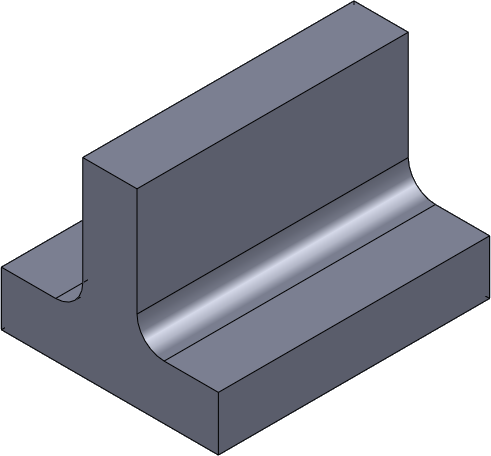
\includegraphics[height=1.5cm]{png/encastrement_sw}
\end{center}
%&
%&
&  
&$$\torseurc{\mathcal{V}\left(S_2/S_1\right)}{\quad}{}{}{}{}{}{\_}$$\\
\hline
\begin{center}
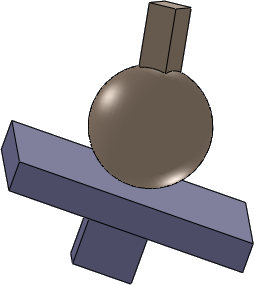
\includegraphics[height=1.5cm]{png/ponctuelle_sw}
\end{center}
& %&
\begin{center}
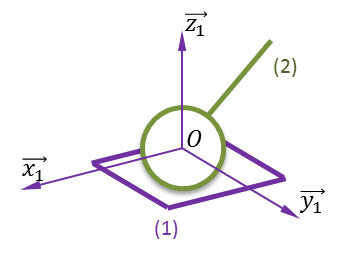
\includegraphics[height=1.5cm]{png/ponctuelle_3d}
\end{center}
%& 
&$$\torseurc{\mathcal{V}\left(S_2/S_1\right)}{\quad}{}{}{}{}{}{\_}$$\\
\hline
\begin{center}
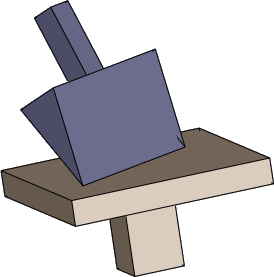
\includegraphics[height=1.5cm]{png/rectiligne_sw}
\end{center}
& %&
\begin{center}
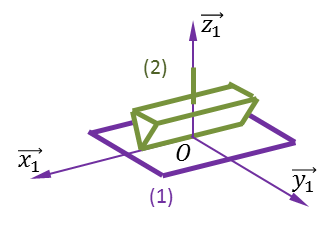
\includegraphics[height=1.5cm]{png/rectiligne_3d}
\end{center}
%& 
&$$\torseurc{\mathcal{V}\left(S_2/S_1\right)}{\quad}{}{}{}{}{}{\_}$$\\
\hline
\begin{center}
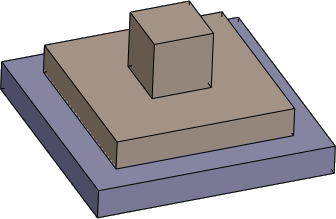
\includegraphics[height=1.5cm]{png/plan_sw}
\end{center}
& %&
\begin{center}
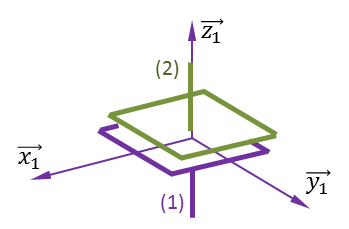
\includegraphics[height=1.5cm]{png/plan_3d}
\end{center}
%& 
&$$\torseurc{\mathcal{V}\left(S_2/S_1\right)}{\quad}{}{}{}{}{}{\_}$$\\
\hline
\begin{center}
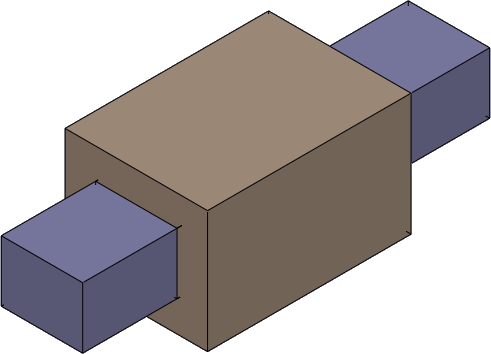
\includegraphics[height=1.5cm]{png/glissiere_sw}
\end{center}
& %&
\begin{center}
\includegraphics[height=1.5cm]{png/glissiere_3d}
\end{center}
%& 
&$$\torseurc{\mathcal{V}\left(S_2/S_1\right)}{\quad}{}{}{}{}{}{\_}$$\\
\hline
\end{tabular}}
\end{center}


\begin{center}\rotatebox{90}{
%\begin{tabular}{|p{.15\textwidth}|p{.1\textwidth}|p{.1\textwidth}|p{.1\textwidth}|p{.22\textwidth}|}
\begin{tabular}{|p{.15\textwidth}|p{.12\textwidth}|p{.22\textwidth}|}
\hline
% & 
%\begin{center}
%Schémas plans
%\end{center} 
& 
%\begin{center}
Schéma spatial
%\end{center} 
& 
%\begin{center}
%DDL 
%\end{center}& 
%\begin{center}
Torseur cinématique 
%\end{center} 
\\
\hline
\hline
\begin{center}
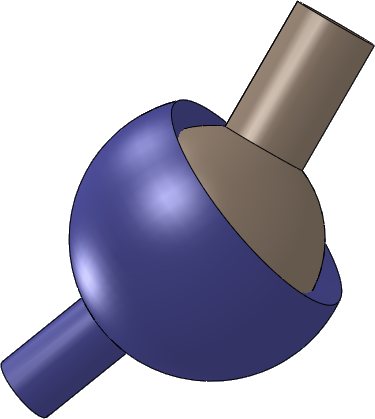
\includegraphics[height=1.5cm]{png/rotule_sw}
\end{center}
& %&
\begin{center}
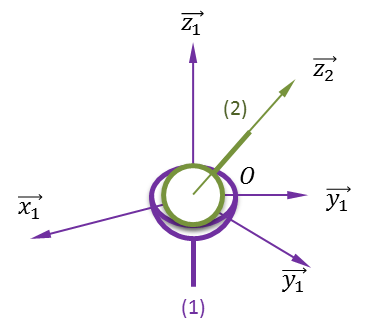
\includegraphics[height=1.5cm]{png/rotule_3d}
\end{center}
%&  
&$$\torseurc{\mathcal{V}\left(S_2/S_1\right)}{\quad}{}{}{}{}{}{\_}$$\\
\hline
\begin{center}
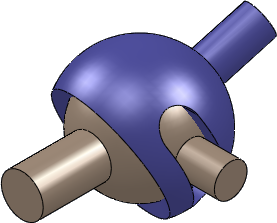
\includegraphics[height=1.5cm]{png/rotuled_sw}
\end{center}
& %&
%\begin{center}
%\includegraphics[height=1.5cm]{png/rotuled_3d}
%\end{center}
%& 
&$$\torseurc{\mathcal{V}\left(S_2/S_1\right)}{\quad}{}{}{}{}{}{\_}$$\\
\hline
\begin{center}
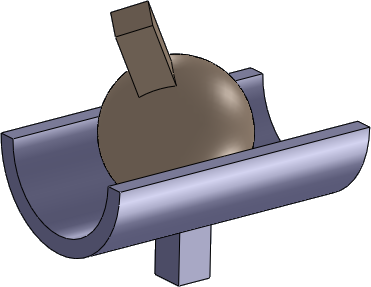
\includegraphics[height=1.5cm]{png/lineaire_sw}
\end{center}
& %&
\begin{center}
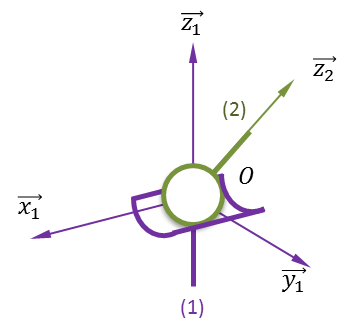
\includegraphics[height=1.5cm]{png/annulaire_3d}
\end{center}
%& 
&$$\torseurc{\mathcal{V}\left(S_2/S_1\right)}{\quad}{}{}{}{}{}{\_}$$\\
\hline
\begin{center}
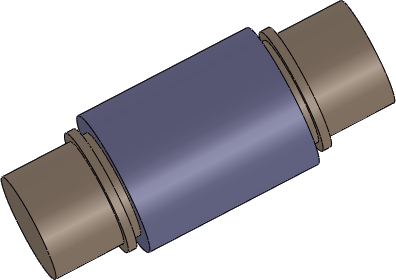
\includegraphics[height=1.5cm]{png/pivot_sw}
\end{center}
& %&
\begin{center}
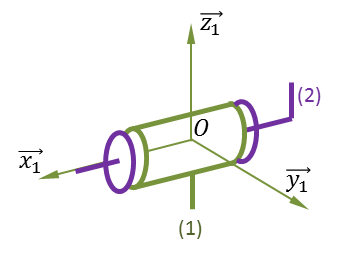
\includegraphics[height=1.5cm]{png/pivot_3d}
\end{center}
% & 
&$$\torseurc{\mathcal{V}\left(S_2/S_1\right)}{\quad}{}{}{}{}{}{\_}$$\\
\hline
\begin{center}
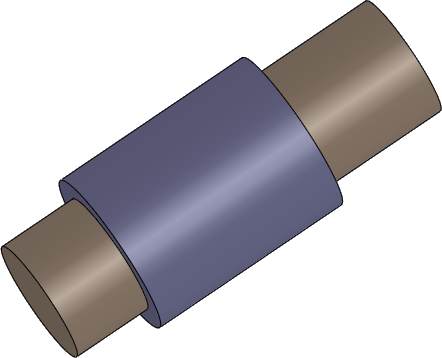
\includegraphics[height=1.5cm]{png/pivotg_sw}
\end{center}
&% &
\begin{center}
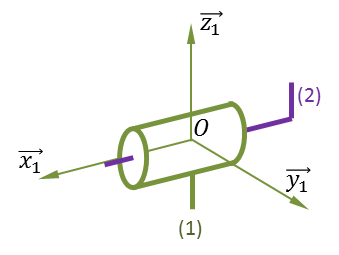
\includegraphics[height=1.5cm]{png/pivotg_3d}
\end{center}
%& 
&$$\torseurc{\mathcal{V}\left(S_2/S_1\right)}{\quad}{}{}{}{}{}{\_}$$\\
\hline
\begin{center}
Liaison glissière hélicoïdale
%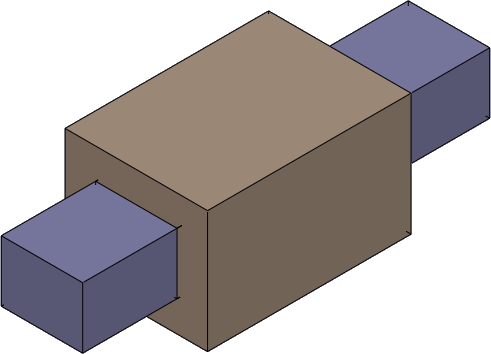
\includegraphics[height=1.5cm]{png/glissiere}
\end{center}
& %&
\begin{center}
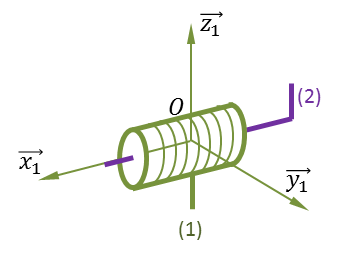
\includegraphics[height=1.5cm]{png/helico_3d}
\end{center}
% & 
&$$\torseurc{\mathcal{V}\left(S_2/S_1\right)}{\quad}{}{}{}{}{}{\_}$$\\
\hline
\end{tabular}}
\end{center}


\subsection{Composition du torseur cinématique}
\begin{resultat}
\textbf{Composition du torseur cinématique}

Le vecteur vitesse et le vecteur instantané pouvant être décomposés, on a donc :

$$
\torseurcin{V}{S_n}{S_0} = 
\torseurcin{V}{S_n}{S_{n-1}} +... +\torseurcin{V}{S_1}{S_0}
$$

Ou encore : 

$$
\torseurl{\vecto{S_n}{S_0}}{\vectv{A}{S_n}{S_0}}{A}=
\torseurl{\vecto{S_n}{S_{n-1}}}{\vectv{A}{S_n}{S_{n-1}}}{A}
+...+
\torseurl{\vecto{S_1}{S_0}}{\vectv{A}{S_1}{S_0}}{A}
$$

\end{resultat}


\section{Torseur des petits déplacements}
\subsection{Définition}
Le torseur cinématique est un outil permettant de modéliser les <<~grands déplacements~>> entre deux solides. Cependant, dans une liaison cinématique, peuvent exister de petits déplacements comme les jeux. 

Les petits déplacements sont notés ainsi : 
\begin{itemize}
\item $\delta u_x$ petit déplacement en translation suivant l'axe $\vect{x}$;
\item $\delta u_y$ petit déplacement en translation suivant l'axe $\vect{y}$;
\item $\delta u_z$ petit déplacement en translation suivant l'axe $\vect{z}$;
\item $\delta \theta_x$ petit déplacement en rotation autour de l'axe $\vect{x}$;
\item $\delta \theta_y$ petit déplacement en rotation autour de l'axe $\vect{y}$;
\item $\delta \theta_z$ petit déplacement en rotation autour de l'axe $\vect{z}$.
\end{itemize}

\begin{defi}
\textbf{Torseur des petits déplacements}

On note $\torseur{\mathcal{U}(S_2/S_1)}$ le torseurs des petits déplacements existants entre deux solides $S_2$ et $S_1$. On a : 
$$\torseur{\mathcal{U}(S_2/S_1)}
=
\torseurl{\delta \theta_x \vect{x} +\delta \theta_y \vect{y} +\delta \theta_z \vect{z} }{
\delta u_x \vect{x} +\delta u_y \vect{y} +\delta u_z \vect{z}}{P}
=\torseurcol{\delta \theta_x}{\delta \theta_y}{\delta \theta_z}{\delta u_x}{\delta u_y}{\delta u_z}{P,\mathcal{R}}
$$
\end{defi}


\subsection{Torseurs des petits déplacements des liaisons usuelles}
Partant de la définition du torseur des petits déplacements et de la connaissance du comportement cinématique des liaisons, il est aisé d'écrire le torseur associé à chacune des liaisons.


\ifthenelse{\boolean{prof}}{
\begin{center}
%\begin{tabular}{|p{.15\textwidth}|p{.1\textwidth}|p{.1\textwidth}|p{.1\textwidth}|p{.22\textwidth}|}
\rotatebox{90}{
\begin{tabular}{|m{.15\textwidth}|m{.12\textwidth}|m{.22\textwidth}|}
\hline
% & 
%\begin{center}
%Schémas plans
%\end{center} 
& 
%\begin{center}
Schéma 3d
%\end{center}
%& 
%\begin{center}
%DDL 
%\end{center}
& 
%\begin{center}
Torseur petits dép. 
%\end{center} 
\\
\hline
\hline
\begin{center}
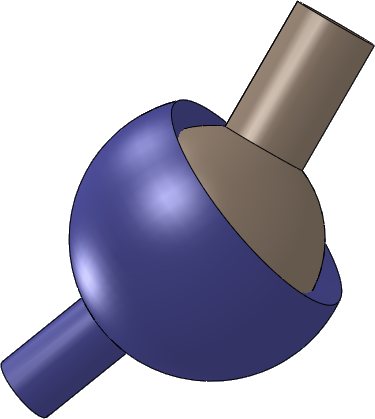
\includegraphics[height=1.5cm]{png/rotule_sw}
\end{center}
& %&
\begin{center}
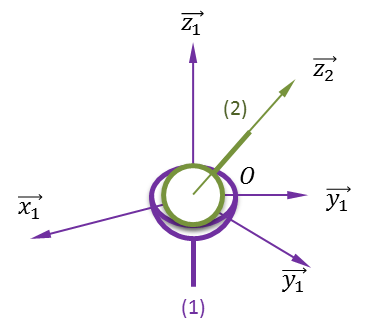
\includegraphics[height=1.5cm]{png/rotule_3d}
\end{center}
%&  
&$$\torseurc{\mathcal{U}\left(S_2/S_1\right)}{\quad}{}{}{}{}{}{\_}$$\\
\hline
\begin{center}
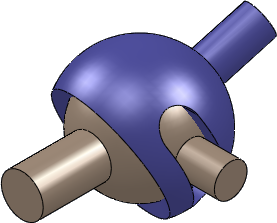
\includegraphics[height=1.5cm]{png/rotuled_sw}
\end{center}
& %&
%\begin{center}
%\includegraphics[height=1.5cm]{png/rotuled_3d}
%\end{center}
%& 
&$$\torseurc{\mathcal{U}\left(S_2/S_1\right)}{\delta \theta_x}{\delta \theta_y}{\delta \theta_z}{}{}{}{\_}$$\\
\hline
\begin{center}
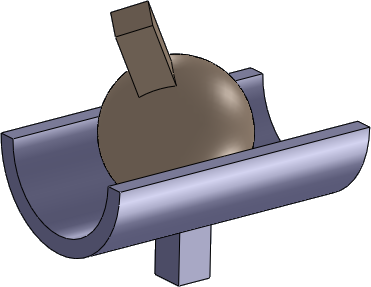
\includegraphics[height=1.5cm]{png/lineaire_sw}
\end{center}
& %&
\begin{center}
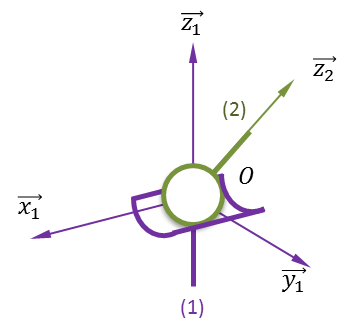
\includegraphics[height=1.5cm]{png/annulaire_3d}
\end{center}
%& 
&$$\torseurc{\mathcal{U}\left(S_2/S_1\right)}{\delta \theta_x}{\delta \theta_y}{\delta \theta_z}{}{}{}{\_}$$\\
\hline
\begin{center}
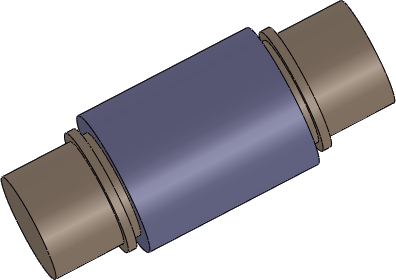
\includegraphics[height=1.5cm]{png/pivot_sw}
\end{center}
& %&
\begin{center}
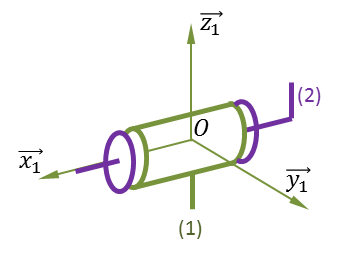
\includegraphics[height=1.5cm]{png/pivot_3d}
\end{center}
% & 
&$$\torseurc{\mathcal{U}\left(S_2/S_1\right)}{\quad}{}{}{}{}{}{\_}$$\\
\hline
\begin{center}
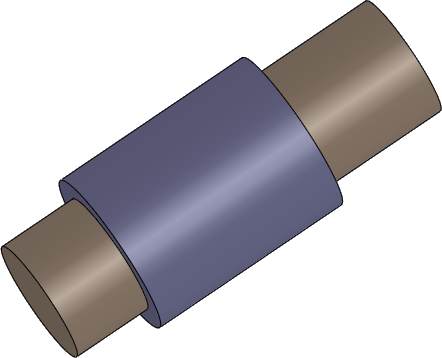
\includegraphics[height=1.5cm]{png/pivotg_sw}
\end{center}
&% &
\begin{center}
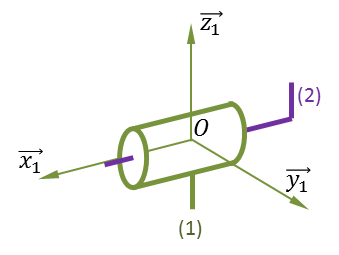
\includegraphics[height=1.5cm]{png/pivotg_3d}
\end{center}
%& 
&$$\torseurc{\mathcal{U}\left(S_2/S_1\right)}{\quad}{}{}{}{}{}{\_}$$\\
\hline
\begin{center}
Liaison glissière hélicoïdale
%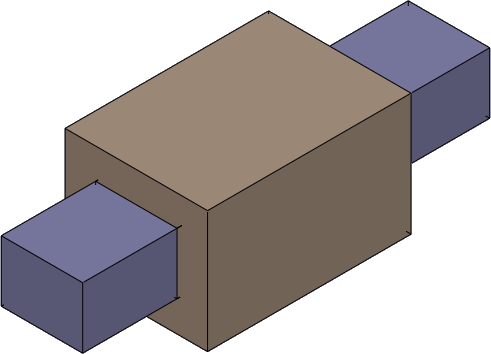
\includegraphics[height=1.5cm]{png/glissiere}
\end{center}
& %&
\begin{center}
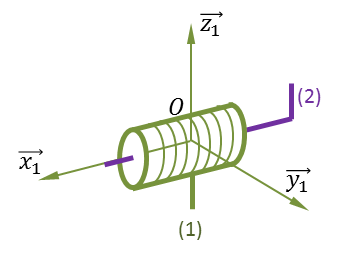
\includegraphics[height=1.5cm]{png/helico_3d}
\end{center}
% & 
&$$\torseurc{\mathcal{U}\left(S_2/S_1\right)}{\quad}{}{}{}{}{}{\_}$$\\
\hline
\end{tabular}}
\end{center}


\begin{center}\rotatebox{90}{
%\begin{tabular}{|p{.15\textwidth}|p{.1\textwidth}|p{.1\textwidth}|p{.1\textwidth}|p{.22\textwidth}|}
\begin{tabular}{|p{.15\textwidth}|p{.12\textwidth}|p{.22\textwidth}|}
\hline
% & 
%\begin{center}
%Schémas plans
%\end{center} 
& 
%\begin{center}
Schéma 3d
%\end{center} 
& 
%\begin{center}
%DDL 
%\end{center}& 
%\begin{center}
Torseur petits dep.
%\end{center} 
\\
\hline
\hline
\begin{center}
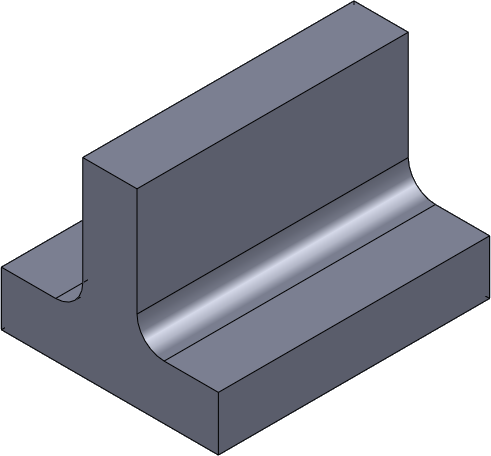
\includegraphics[height=1.5cm]{png/encastrement_sw}
\end{center}
%&
%&
&  
&$$\torseurc{\mathcal{U}\left(S_2/S_1\right)}{\quad}{}{}{}{}{}{\_}$$\\
\hline
\begin{center}
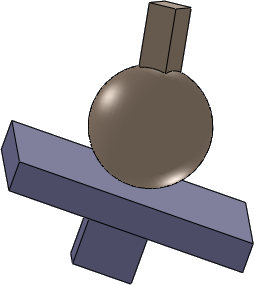
\includegraphics[height=1.5cm]{png/ponctuelle_sw}
\end{center}
& %&
\begin{center}
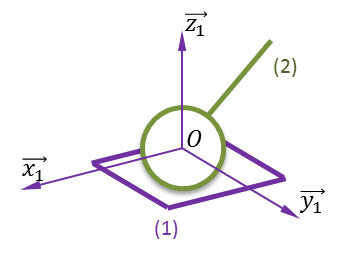
\includegraphics[height=1.5cm]{png/ponctuelle_3d}
\end{center}
%& 
&$$\torseurc{\mathcal{U}\left(S_2/S_1\right)}{\quad}{}{}{}{}{}{\_}$$\\
\hline
\begin{center}
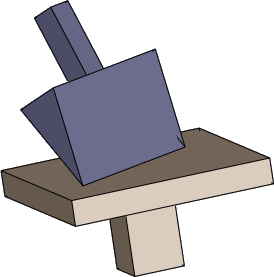
\includegraphics[height=1.5cm]{png/rectiligne_sw}
\end{center}
& %&
\begin{center}
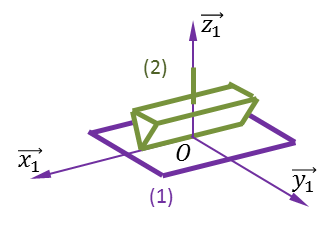
\includegraphics[height=1.5cm]{png/rectiligne_3d}
\end{center}
%& 
&$$\torseurc{\mathcal{U}\left(S_2/S_1\right)}{\quad}{}{}{}{}{}{\_}$$\\
\hline
\begin{center}
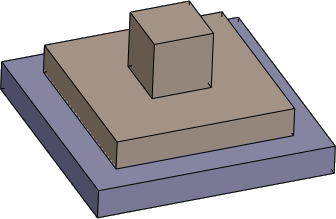
\includegraphics[height=1.5cm]{png/plan_sw}
\end{center}
& %&
\begin{center}
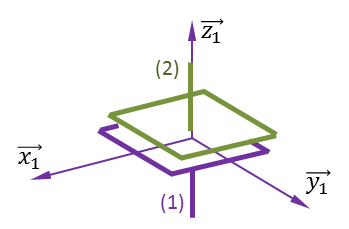
\includegraphics[height=1.5cm]{png/plan_3d}
\end{center}
%& 
&$$\torseurc{\mathcal{U}\left(S_2/S_1\right)}{\quad}{}{}{}{}{}{\_}$$\\
\hline
\begin{center}
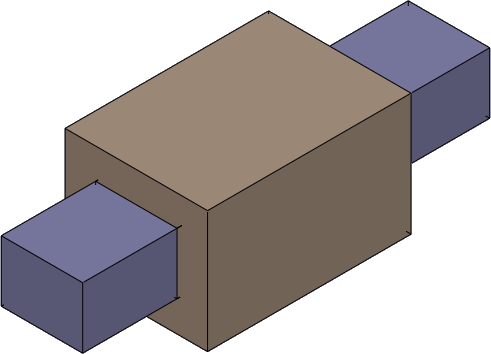
\includegraphics[height=1.5cm]{png/glissiere_sw}
\end{center}
& %&
\begin{center}
\includegraphics[height=1.5cm]{png/glissiere_3d}
\end{center}
%& 
&$$\torseurc{\mathcal{U}\left(S_2/S_1\right)}{\quad}{}{}{}{}{}{\_}$$\\
\hline
\end{tabular}}
\end{center}


\begin{center}
%\begin{tabular}{|p{.15\textwidth}|p{.1\textwidth}|p{.1\textwidth}|p{.1\textwidth}|p{.22\textwidth}|}
\rotatebox{90}{
\begin{tabular}{|m{.15\textwidth}|m{.12\textwidth}|m{.22\textwidth}|}
\hline
% & 
%\begin{center}
%Schémas plans
%\end{center} 
& 
%\begin{center}
Schéma 3d
%\end{center}
%& 
%\begin{center}
%DDL 
%\end{center}
& 
%\begin{center}
Torseur petits dép. 
%\end{center} 
\\
\hline
\hline
\begin{center}
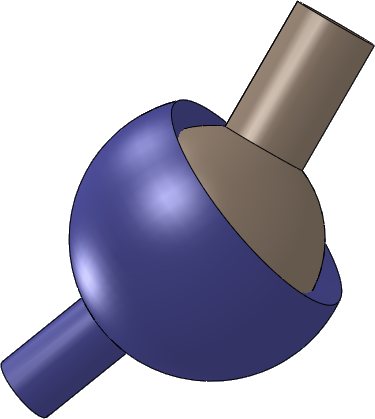
\includegraphics[height=1.5cm]{png/rotule_sw}
\end{center}
& %&
\begin{center}
\includegraphics[height=1.5cm]{png/rotule_3d}
\end{center}
%&  
&$$\torseurc{\mathcal{U}\left(S_2/S_1\right)}{\quad}{}{}{}{}{}{\_}$$\\
\hline
\begin{center}
\includegraphics[height=1.5cm]{png/rotuled_sw}
\end{center}
& %&
%\begin{center}
%\includegraphics[height=1.5cm]{png/rotuled_3d}
%\end{center}
%& 
&$$\torseurc{\mathcal{U}\left(S_2/S_1\right)}{\quad}{}{}{}{}{}{\_}$$\\
\hline
\begin{center}
\includegraphics[height=1.5cm]{png/lineaire_sw}
\end{center}
& %&
\begin{center}
\includegraphics[height=1.5cm]{png/annulaire_3d}
\end{center}
%& 
&$$\torseurc{\mathcal{U}\left(S_2/S_1\right)}{\quad}{}{}{}{}{}{\_}$$\\
\hline
\begin{center}
\includegraphics[height=1.5cm]{png/pivot_sw}
\end{center}
& %&
\begin{center}
\includegraphics[height=1.5cm]{png/pivot_3d}
\end{center}
% & 
&$$\torseurc{\mathcal{U}\left(S_2/S_1\right)}{\quad}{}{}{}{}{}{\_}$$\\
\hline
\begin{center}
\includegraphics[height=1.5cm]{png/pivotg_sw}
\end{center}
&% &
\begin{center}
\includegraphics[height=1.5cm]{png/pivotg_3d}
\end{center}
%& 
&$$\torseurc{\mathcal{U}\left(S_2/S_1\right)}{\quad}{}{}{}{}{}{\_}$$\\
\hline
\begin{center}
Liaison glissière hélicoïdale
%\includegraphics[height=1.5cm]{png/glissiere}
\end{center}
& %&
\begin{center}
\includegraphics[height=1.5cm]{png/helico_3d}
\end{center}
% & 
&$$\torseurc{\mathcal{U}\left(S_2/S_1\right)}{\quad}{}{}{}{}{}{\_}$$\\
\hline
\end{tabular}}
\end{center}
}{\begin{center}\rotatebox{90}{
%\begin{tabular}{|p{.15\textwidth}|p{.1\textwidth}|p{.1\textwidth}|p{.1\textwidth}|p{.22\textwidth}|}
\begin{tabular}{|p{.15\textwidth}|p{.12\textwidth}|p{.22\textwidth}|}
\hline
% & 
%\begin{center}
%Schémas plans
%\end{center} 
& 
%\begin{center}
Schéma 3d
%\end{center} 
& 
%\begin{center}
%DDL 
%\end{center}& 
%\begin{center}
Torseur petits dep.
%\end{center} 
\\
\hline
\hline
\begin{center}
\includegraphics[height=1.5cm]{png/encastrement_sw}
\end{center}
%&
%&
&  
&$$\torseurc{\mathcal{U}\left(S_2/S_1\right)}{\quad}{}{}{}{}{}{\_}$$\\
\hline
\begin{center}
\includegraphics[height=1.5cm]{png/ponctuelle_sw}
\end{center}
& %&
\begin{center}
\includegraphics[height=1.5cm]{png/ponctuelle_3d}
\end{center}
%& 
&$$\torseurc{\mathcal{U}\left(S_2/S_1\right)}{\quad}{}{}{}{}{}{\_}$$\\
\hline
\begin{center}
\includegraphics[height=1.5cm]{png/rectiligne_sw}
\end{center}
& %&
\begin{center}
\includegraphics[height=1.5cm]{png/rectiligne_3d}
\end{center}
%& 
&$$\torseurc{\mathcal{U}\left(S_2/S_1\right)}{\quad}{}{}{}{}{}{\_}$$\\
\hline
\begin{center}
\includegraphics[height=1.5cm]{png/plan_sw}
\end{center}
& %&
\begin{center}
\includegraphics[height=1.5cm]{png/plan_3d}
\end{center}
%& 
&$$\torseurc{\mathcal{U}\left(S_2/S_1\right)}{\quad}{}{}{}{}{}{\_}$$\\
\hline
\begin{center}
\includegraphics[height=1.5cm]{png/glissiere_sw}
\end{center}
& %&
\begin{center}
\includegraphics[height=1.5cm]{png/glissiere_3d}
\end{center}
%& 
&$$\torseurc{\mathcal{U}\left(S_2/S_1\right)}{\quad}{}{}{}{}{}{\_}$$\\
\hline
\end{tabular}}
\end{center}
}


\begin{thebibliography}{2}
\bibitem[1]{jpp} Jean-Pierre Pupier, Les Torseurs, Cours de mécanique, lycée Rouvière.
\end{thebibliography}
\end{document}



\end{document}


